\documentclass{article}
% \usepackage{arxiv}

\usepackage[utf8]{inputenc}
% \usepackage[russian]{babel}
\usepackage[english]{babel}
\usepackage[T1]{fontenc}
\usepackage{url}
\usepackage{booktabs}
\usepackage{amsfonts}
\usepackage{nicefrac}
% \usepackage{amsbib}
\usepackage{microtype}
\usepackage{amsthm}

\usepackage{bm}
\usepackage{mathrsfs}
\usepackage{lipsum}
\usepackage{graphicx}
\usepackage{natbib}
\usepackage{wrapfig}
\usepackage{doi}
\newtheorem{theorem}{Theorem}[section]
\newtheorem{corollary}{Corollary}[theorem]

\usepackage{mathtools}
\usepackage{amsmath}
\DeclareMathOperator*{\argmax}{arg\,max}
\DeclareMathOperator*{\argmin}{arg\,min}
\usepackage[dvipsnames]{xcolor}

\title{Inductive Bias in Model Selection}
% Russian title: Выбор предсказательной модели в режиме многозадачного обучения с применением методов символьной регрессии

\author{
    Muhammadsharif Nabiev \\
    Department of Intelligent Systems\\
    MIPT\\
    \texttt{nabiev.mf@phystech.edu} \\
    % \And
    % Oleg Bakhteev \\
    % Department of Intelligent Systems\\
    % MIPT\\
    \texttt{} \\
}
\date{}

% \renewcommand{\shorttitle}{Inductive bias in model selection}

\hypersetup{
pdftitle={Inductive bias in model selection},
pdfsubject={q-bio.NC, q-bio.QM},
pdfauthor={Muhammadsharif},
pdfkeywords={model selection, evolutionary algorithm},
}

\begin{document}
\maketitle

\begin{abstract}
% This paper addresses the challenge of selecting architectures for suboptimal models within the multitask learning paradigm. Given a set of inherently similar tasks, the objective is to identify a shared structure across all tasks — referred to as the inductive bias. Using constrained evolutionary symbolic regression, it can be demonstrated that the models can be decomposed in a manner that reveals the underlying structure of the tasks. We conducted experiments on synthetic data, where we know structure of the data, the process of data generation and optimal models. The results demonstrate that the models obtained by the proposed method are indeed optimal for corresponding tasks.

This paper tackles the problem of constructing suboptimal models within multitask learning paradigm. Given a set of intrinsically related tasks, the goal is to uncover a shared structure—known as the inductive bias—across all tasks. By applying constrained evolutionary symbolic regression, we show that these models can be decomposed in a way that reveals the tasks' underlying structure. We performed experiments on synthetic data, where the data structure, generation process, and optimal models are known. The results indicate that the models produced by the proposed method are indeed optimal for their respective tasks.


% This paper is devoted to the problem of choosing the architecture of suboptimal models in multitask learning paradigm. The assumption is introduced that when searching for models in the search space of a sufficiently high dimension, the resulting model architecture will reflect the features of the analyzed data, which can be interpreted as an inductive bias of the model. An automatic procedure can be employed using evolutionary method of searching for a model based on symbolic regression algorithms. Model trains independently on a set of given datasets of a particular class. 

% Inductive bias играет ключевую роль для обобщения модели, так как разнородные данные имеют свои уникальные отличительные черты, которые отличают одни данные от других. В данной работе мы предлагаем автоматизированный подход к выявлению inductive bias в наборе данных, используя модифицированную версию AutoML-Zero. AutoML-Zero - эволюционный алгоритм, который автоматически проектирует модели для решения задачи на заданных данных. Мы предлагаем следующие модификации \textcolor{red}{need to write more}

% another version 
% This paper addresses the challenge of selecting optimal model architectures within the multitask learning paradigm. We propose that, when exploring model architectures in a high-dimensional search space, the resultant models will inherently reflect the characteristics of the data being analyzed. This phenomenon can be understood as the model's inductive bias. We introduce an automated approach leveraging evolutionary algorithms in combination with symbolic regression to facilitate the search for appropriate models. Our methodology allows models to be trained independently on diverse datasets within a specific class, thus enhancing generalizability and adaptability.

\end{abstract}

% \keywords{model selection \and evolutionary algorithm}

\section{Introduction} 
The concept of inductive bias is a fundamental tenet in the realm of machine learning, encapsulating the core assumptions that underpin the methodology adopted by a particular model in its predictive endeavours, extending beyond the boundaries of explicitly observed data. Understanding and leveraging inductive bias is essential for enhancing model performance, especially in complex environments where data may exhibit diverse characteristics. 

In recent years, the field of machine learning has experienced rapid advancements driven by the development of sophisticated algorithms and architectures capable of tackling a wide range of tasks, from natural language processing to computer vision. However, the design and optimization of these models often require significant expertise and resources, leading to the rise of automated machine learning (AutoML) systems. These systems aim to alleviate the burden of manual model selection and tuning, enabling broader accessibility to machine learning techniques.

One notable approach is AutoML-Zero, which autonomously constructs models using a genetic programming framework, assembling them from fundamental mathematical operations \citep{automl-zero}. This method represents a significant departure from traditional model selection paradigms, which typically rely on predefined structures or human intuition. By allowing the model architecture to emerge organically from the data, AutoML-Zero minimizes biases introduced by prior knowledge, potentially leading to the discovery of novel architectures better suited to the task at hand.

The concept of inductive bias plays a crucial role in model generalization. Different datasets often possess unique distinguishing features that can be exploited for improved performance. For instance, models trained on image data may benefit from biases related to spatial hierarchies, while those handling sequential data, such as time series or text, may rely on temporal dependencies. Recognizing and systematically integrating these biases into the model selection process can facilitate the identification of suboptimal yet effective architectures.

In this paper, we investigate how inductive biases inherent in the data can inform model selection within the multitask learning framework. We propose an automated approach that leverages evolutionary algorithms in conjunction with symbolic regression to explore a diverse range of model architectures. By allowing models to train independently on various datasets within a specific class, our methodology aims to enhance generalizability and adaptability while reducing the need for extensive manual tuning.

The experiments are focused on a range of datasets that capture different characteristics, enabling a robust evaluation of how well our models generalize across tasks. The goal is to provide insights into the relationship between inductive bias and model architecture.
\citep{Cranmer2023InterpretableML}
\newline 
About inductive bias, multitask, symbolic regression, info bottleneck, and llm interpretability. 
\newline
    
% \begin{figure}[hbt!]
%     \centering
%     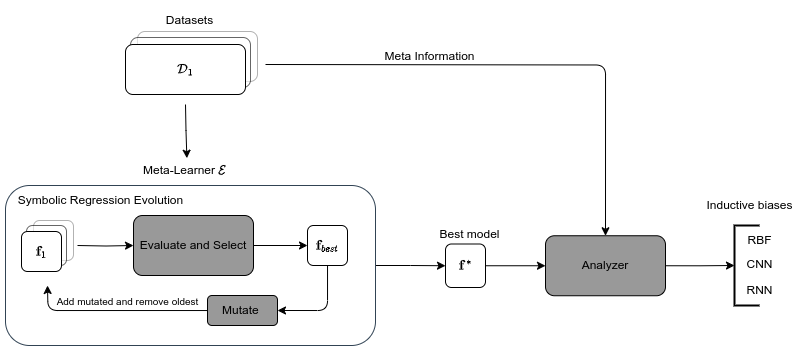
\includegraphics[width=1\textwidth]{model.png}
%     \caption{Pipeline.}
%     \label{pipeline}
% \end{figure}
\begin{figure}[hbt!]
    \centering
    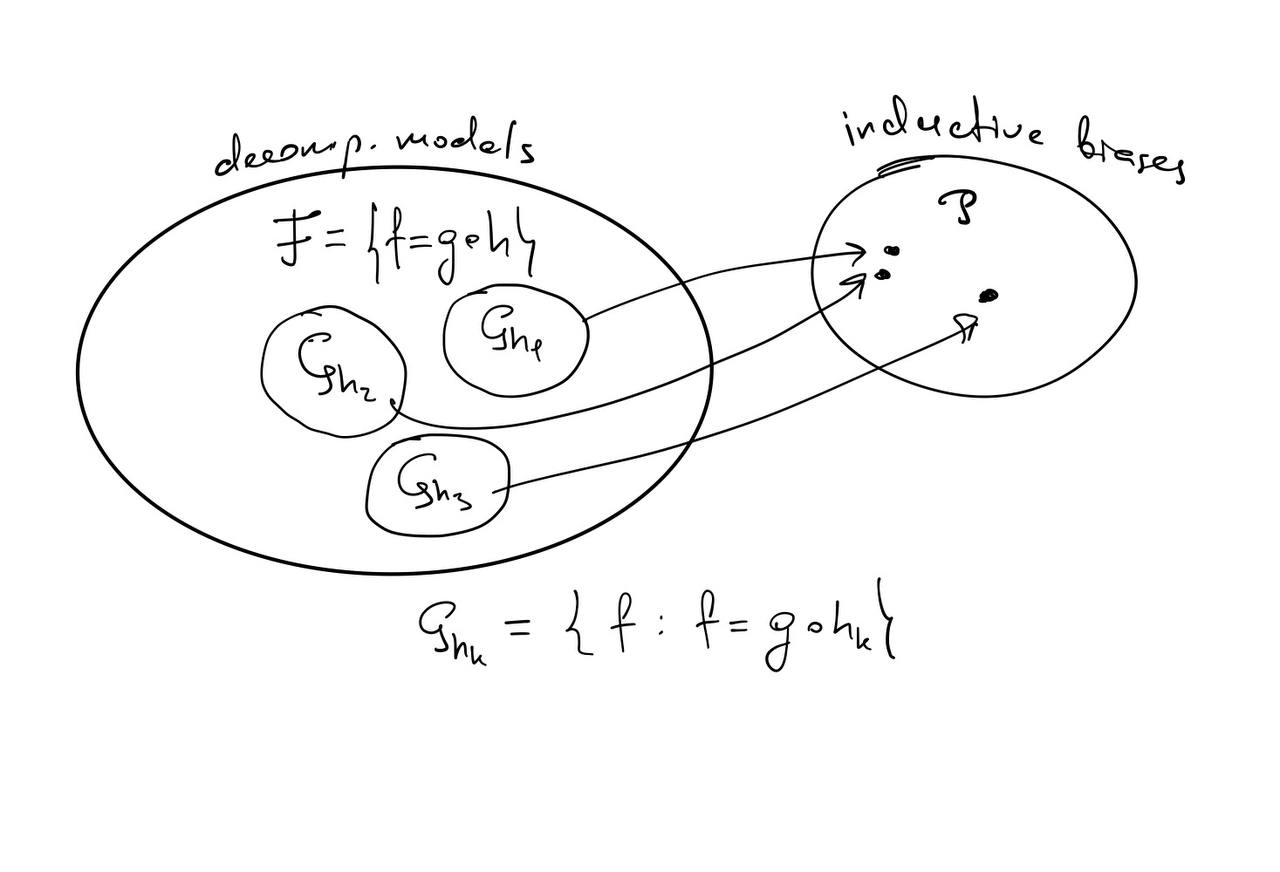
\includegraphics[width=1\textwidth]{sets.jpg}
    \caption{Models coresponding to inductive biases.}
    \label{pipeline}
\end{figure}

\section{Problem statement}
    Let \( \mathfrak{T} = \{T_1, T_2, \dots, T_n\} \) be a set of tasks. Each task \( T_i \) has its corresponding dataset \( \mathfrak{D}_i = \{(\mathbf{x}_j, \mathbf{y}_j) \}_{j=1}^{N_i} \) with and object \(\mathbf{x}_j\) and a label \(\mathbf{y}_j\).
    
    A \textit{model} \(\mathbf{f}\) is defined as an expression with the following mapping \(\mathbb{R}^n \rightarrow \mathbb{R}^m\), whose \textit{structure} \(\Gamma\) can be represented via expression tree~\citep{RudStr13}. In search of such models, we will employ an evolutionary search algorithm to discover a general model — up to constant factors — that can address the tasks \(\mathfrak{T}\). 
    
    Let \(\mathfrak{F}\) be a parametric family of all models which can be decomposed as such \(\mathbf{f} = \mathbf{g} \circ \mathbf{h}\), where \(\mathbf{g}\) and \(\mathbf{h}\) will be referred to as \textit{decoder} and \textit{encoder}. It is also worth noting that any \(\mathbf{f}\) can be decomposed in the prescribed way.
    \begin{theorem}\label{decomposition}
        For any expression \(\mathbf{f}: \mathbb{R}^n \rightarrow \mathbb{R}^m\) there exists \(\mathbf{h}:\mathbb{R}^n\rightarrow \mathbb{R}^d\) and \(\mathbf{g}:\mathbb{R}^d\rightarrow \mathbb{R}^m\) such that \(\mathbf{f} = \mathbf{g} \circ \mathbf{h}\).
    \end{theorem}
    \begin{proof}
        Trivial cases:
        \begin{itemize}
            \item \(d = m\). We take \(\mathbf{h} = \mathbf{f}\) and \(\mathbf{g} = \operatorname{Id}\), hence \(\mathbf{f}(\mathbf{x}) = \mathbf{g}(\mathbf{h}(\mathbf{x})) = \mathbf{g}(\mathbf{f}(\mathbf{x})) = \mathbf{f}(\mathbf{x})\).
            \item \(d = n\). We take \(\mathbf{h}=\operatorname{Id}\) and \(\mathbf{g}=\mathbf{f}\), hence \(\mathbf{f}(\mathbf{x}) = \mathbf{g}(\mathbf{h}(\mathbf{x})) = \mathbf{g}(\mathbf{x}) = \mathbf{f}(\mathbf{x})\)
        \end{itemize}
        For non-trivial cases the decomposition can be obtained using Kolmogorov-Arnold theorem~\cite{kolmogorov1961representation}. 
    \end{proof}

    By the nature of the given decomposition we have to put restrictions on encoder, otherwise when certain conditions are fulfilled we can fall into degenerate cases for the structure of the decoder.
    \begin{theorem}\label{bottleneck_dim}
        Let \(\mathbf{f}:\mathbb{R}^n \rightarrow \mathbb{R}^m\). For a latent space \(\mathbb{R}^d\) such that \(d \ge m\) we can construct a decomposition \(\mathbf{f} = \mathbf{g} \circ \mathbf{h}\) such that \(\mathbf{g} = \operatorname{Id}_Z\) and \(Z \cong \mathbb{R}^m\).
    \end{theorem}
    \begin{proof}
        Since \(m \le d\) we can redefine latent space as \(Z \cong \mathbb{R}^m\) and the given expression \(\mathbf{f}\) by ignoring extra dimensions. If we take \(\mathbf{h} = \mathbf{f} : \mathbb{R}^n \rightarrow Z\) and \(\mathbf{g} = \operatorname{Id}_{Z}\) we get \(\mathbf{f}(\mathbf{x}) = \mathbf{g}(\mathbf{h}(\mathbf{x})) = \operatorname{Id}_{Z} (\mathbf{f}(\mathbf{x})) = \mathbf{f}(\mathbf{x})\).
    \end{proof}

    By Theorem~\ref{bottleneck_dim} it follows that we have to restrict the dimensionality of a latent space. In order to do that we incorporate \textit{Information Bottleneck} method.
    
    \subsection{Information Bottleneck}        
        A statistic \(\operatorname{S}(\mathbf{X})\) is called \textit{sufficient} if the mutual information between \(\operatorname{S}(\mathbf{X})\) and \(\mathbf{Y}\) is the same as the mutual information between \(\mathbf{X}\) and \(\mathbf{Y}\), i.e. \(\operatorname{I}(\mathbf{X}, \mathbf{Y}) = \operatorname{I}(\operatorname{S}(\mathbf{X}), \mathbf{Y})\). A sufficient statistic is called \textit{minimal} if it minimizes information about input data \(\mathbf{X}\):
        \[
            \operatorname{T}(\mathbf{X}) = \argmin_{\operatorname{S}(X): \operatorname{I}(\operatorname{S}(\mathbf{X}), \mathbf{Y}) = \operatorname{I}(\mathbf{X}, \mathbf{Y})} \operatorname{I}(\operatorname{S}(\mathbf{X}), \mathbf{X}).
        \]
        
        Information bottleneck principle aims to find an internal representation that maximizes information about \(\mathbf{Y}\) while minimizing information about \(\mathbf{X}\), i.e.
        \[
            \min_{p(T | \mathfrak{D})} \operatorname{I}(\mathbf{X}, \operatorname{T}(\mathbf{X})) - \beta \operatorname{I}(\operatorname{T}(\mathbf{X}), \mathbf{Y}).
        \]
            
        Suppose \(\mathcal{L}_{\text{task}}\) is a loss of the task being solved. It is worth noting that the task-loss could not be differentiable. Taking informational bottleneck approach into account we get the final optimization function:
    
    
        \begin{align*}
            \Gamma = &\; \argmin_{f = g \circ h: \; \Gamma - \text{structure of} \; h} \mathbb{E}_{\mathfrak{D}} \mathcal{L}_{\text{task}}(f(X), Y) \\ 
            & \text{s.t.} \; \beta \operatorname{I}(h, Y) - \operatorname{I}(X, h) \rightarrow \max
        \end{align*}

        We define \textit{inductive bias} as the structure of \(\mathbf{h}\). The goal is to construct models which general form can approximate the given tasks. In order to favor generalization an informational bottleneck approach was taken. 
% \hline

        Having multi-task paradigm is crucial for our decomposition. Single-task setting will degenerate our solution to having \(\mathbf{g}=\operatorname{Id}\). 
        \begin{theorem}\label{single_task}
            For single-task paradigm there exists a solution \(\mathbf{f}\) that has a decomposition \(\mathbf{f} = \mathbf{g} \circ \mathbf{h}\), where \(\mathbf{g} = \operatorname{Id}\) and \(\mathbf{h} = \mathbf{f}\).
        \end{theorem}
        \begin{proof}
            For single-task paradigm the optimal solution \(\mathbf{f}\) can itself represent the encoder \(h\). Hence \(\mathbf{h} = \mathbf{f}\) and \(\mathbf{g}=\operatorname{Id}\).
        \end{proof}
        Theorem~\ref{single_task} immediately gives us the following corollary.
        \begin{corollary}
            For multi-task paradigm where all tasks can be generalized by single \(\mathbf{f}\), there exists a solution with \(\mathbf{g}=\operatorname{Id}\).
        \end{corollary}
% Let \(\mathfrak{F}\) be the family of all models. The model is defined by three functions: \texttt{Setup}, \texttt{Learn} and \texttt{Predict}. The meta-learner \(\mathcal{E}: 2^{\mathfrak{D}} \rightarrow \mathfrak{F}\) is based on AutoML-Zero algorithm. The algorithm incorporates evolutionary search method on training datasets to generate candidate models, which are then selected and mutated based on their accuracy on test datasets. Evolutionary search is conducted as follows:
% \begin{itemize}
%     \item Initialization: Generate an initial population of models \( \mathcal{F}_0 \subset \mathfrak{F} \) of size \(P\).
%     \item Evaluation: During each evolution cycle asses each model \( f \in \mathcal{F}_t \) using accuracy metric, where \(\mathcal{F}_t\) is the population at t-th cycle.
%     \item Mutation: Select the best model and mutate it to product a child model. To keep the population size fixed, the oldest model is replaced by the child model. (details about mutation can be put in apendix)
%     \item Termination: Repeat for \(C\) cycles and select the best model \( f^* \) accross all cycles.
% \end{itemize}
% The best model is found based on mean accuracy. If we have \(m_2\) test datasets then the metric on a set of tasks can be computed as 
% \[
%  \operatorname{mACC}(f, \mathfrak{D}) = \frac{1}{m_2} \sum_{i = 1}^{m_2} \operatorname{ACC}(f, \mathfrak{D}_i)
%     = \frac{1}{m_2} \sum_{i=1}^{m_2} \sum_{j=1}^{N_i} \frac{[f(\mathbf{x}_j) = y_j]}{N_i}
% \]
% Hence, the optimization in this stage can be written as 
% \[
%     f^* = \arg \max_{f \in \mathfrak{F}} \operatorname{mACC}(f, \mathfrak{D}).
% \]

% \subsection{Analyzer}
% After construction of an optimal model \(\mathbf{f}^*\) we will utilize LLM to interpret it. The procedure is the following:
% \begin{itemize}
    % \item 
% \end{itemize}
% Given the best model \(\mathbf{f}^*\) we can infer an inductive bias of the tasks. We categorized inductive biases into three categories: RBF, CNN and RNN. The inference is done by analyzer \(\mathbf{f}_{\text{CLF}}\) which was selected to be [MODEL] model. 

% By getting an internal represention of the best model \(f^*\), i.e. the funcitons comprising \texttt{Setup}, \texttt{Predict} and \texttt{Learn}, we use [MODEL] to infer the inductive bias hidden in the representation. 

% OR. Try to make map internal representation of the funcitons into latent space. Maybe functinos with the same inductive biases will cluster?

% Let \( \mathcal{F} \) be the family of all models. The meta-learner \( \mathcal{E} : 2^D \rightarrow \mathcal{F}  \) is based on AutoML-Zero algorithm. Given train datasets \(D_{train} \subset D = \{D_1, D_2, \dots, D_n \}\) the meta-learner \(\mathcal{E}\) generates candidate models \( \{ f_1, f_2, \dots, f_{P}\} \), which are then evaluated on test datasets \(D_{test} \subset D\). The best model \(f_i\) is selected based on mean accuracy and mutated to produce a child algorithm. 



% Let \( \mathfrak{T} = \{T_1, T_2, \dots, T_n\} \) be a set tasks. Each task \( T_i \) has its corresponding dataset \( \mathfrak{D}_i \), where \( \mathfrak{D}_i = \{(\mathbf{x}_j, y_j) \}_{j=1}^{N_i} \) represents \( N_i \) examples of input-output pairs. We will denote meta-learner as \( \mathcal{E} \) and \( \mathcal{M} \) as a space of all possible models. The task is to classify the bias of the given tasks \(\mathfrak{T}\).

% Let \( \mathcal{F} \) be the family of all models. The meta-learner \( \mathcal{E} : 2^D \rightarrow \mathcal{F}  \) is based on AutoML-Zero algorithm. Given train datasets \(D_{train} \subset D = \{D_1, D_2, \dots, D_n \}\) the meta-learner \(\mathcal{E}\) generates candidate models \( \{ f_1, f_2, \dots, f_{P}\} \), which are then evaluated on test datasets \(D_{test} \subset D\). The best model \(f_i\) is selected based on mean accuracy and mutated to produce a child algorithm. 

% Classifier \( \operatorname{Clf} \) aims to extract inductive bias from models , i.e. \( \operatorname{Clf}(f_1, f_2, \dots, f_n) = \hat{b} \). (AutoML-Zero for classifier too?).

% To facilitate model search, we utilize an evolutionary algorithm \( \mathcal{E} \) that iteratively explores and refines potential architectures based on their performance on a given task. The evolutionary process can be summarized as:

% \begin{itemize}
%     \item Initialization: Generate an initial population of models \( P_0 \subset \mathcal{M} \).
%     \item Evaluation: Asses each model \( M \in P_t \) using appropriate loss function or metric.
%     \item Selection: Select a subset of models based on their score.
%     \item Mutation: Apply genetic operations to produce a new generation of models \( P_{t+1} \).
%     \item Termination: Repeat until convergence criteria are met, yielding the final model architecture \( M*\).
% \end{itemize}

% Thus, the core of our problem is to efficiently navigate the architecture space \( \mathcal{M} \), guided by inductive bias \(b\), in order to discover the best models. 

% \section{Model description} 
% The PySR library~\citep{Cranmer2023InterpretableML} as a meta-learner to infer models. Utilizing library's flexible API custom loss functions were introduced for every task. 

\section{Computational experiment}
We used PySR library for to construct model using evolutionary search~\citep{Cranmer2023InterpretableML}. The experiments were conducted on binary classification, autoregression and CNN tasks. For each task the meta-learner trained on 1, 2, 5, 10 and 15 datasets. To incorporate our objective we specified custom loss along with template expression to extract the mapping \(\mathbf{h}\).

    We conduct experiments on three types of data modalities: tabular, sequential and image-based. 
    \subsection{Data}
    % The following tasks were selected: binary classification with a circle as decision boundary and time-series prediction.
    % Suppose \(\{ \mathfrak{D}_1, \mathfrak{D}_2, \dots, \mathfrak{D}_n\} \) are the datasets.
    % The datasets have same inductive bias but they differ from each other by some property.  We select \(m_1\) elements from each dataset to form a set of training datsets \(\mathfrak{D}_{train}\), and from a remaining part we get a set of testing datasets \(\mathfrak{D}_{test}\).
  
    \subsection{Experiments}
    \subsubsection{Tabular}
        We used dataset consisting of circles. Multi-task involved 3 tasks. Binary classification and 2 custom function regressions. 
        
        The decision boundary for datasets was chosed to be a circle for its simplicity and practicality. The circle analitically can be represented as a second-order equation. 
    \subsubsection{Sequential}
        
        Simple AR(1) was chosed to generated synthetic datasets. 

    \subsubsection{Image-based}
        We consider a primitive binary image-tasks with 4/10 pixels. There we must find a distinct pattern

    \subsection{Results of the experiments}

\section{Conclusion}

\bibliographystyle{plain}
\bibliography{ib_in_model_selection}

\end{document}